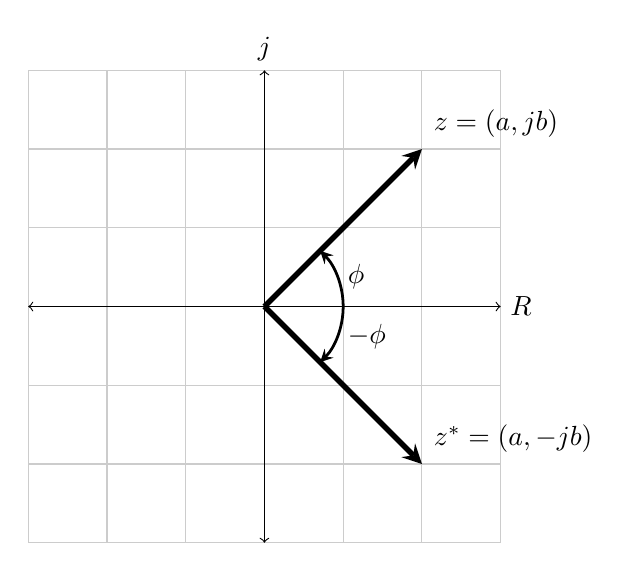
\begin{tikzpicture}
        \draw[thin,gray!40] (-3,-3) grid (3,3);
        \draw[<->] (-3,0)--(3,0) node[right] {$R$};
        \draw[<->] (0,-3)--(0,3) node[above]{$j$};
       \draw[line width=2pt,black,-stealth](0,0)--(2,2) node[anchor=south west]{${z=(a,jb)}$};
       \draw[line width=2pt,black,-stealth](0,0)--(2,-2) node[anchor=south west]{${z^*=(a,-jb)}$};
       \draw[line width=1pt,black,-stealth] (1,0) arc (0:45:1) node [midway, right]{$\phi$};
        \draw[line width=1pt,black,-stealth] (1,0) arc (0:-45:1) node [midway, right]{$-\phi$};
    \end{tikzpicture}
    \caption{conjugado de un numero complejo}